% arara: pdflatex
\documentclass[a4paper]{article}
\usepackage[margin=2.5cm]{geometry}
\usepackage[ngerman]{babel}
\usepackage{syntax}
\usepackage{listings}
\usepackage[dvipsnames]{xcolor}
\usepackage{graphicx}
\usepackage{amssymb}

\title{\textbf{Dokumentation \texttt{picsim}}}

\author{
    Nicolas Dorrmann \\
    Jonas Angene
}

\begin{document}
\maketitle

Das folgende Dokument soll die Funktionsweise eines Simulators für den Mikrocontroller PIC16F84 dokumentieren.
Neben der grundsätzlichen Arbeitsweise eines Simulators werden die wichtigeren Implementierungsdetails besprochen.
Zudem soll eine kurzer Überblick über Funktionen und Verwendung des Simulators gegeben werden.

\section{Simulatoren als Software}

Ein Simulator ist ein Programm, das den Ablauf eines Prozesses simuliert.
Der Prozess ist in diesem Fall der Ablauf einer Reihe von Maschinenbefehlen auf einem Mikrocontroller.
Dabei werden die im Mikrocontroller aufgebauten elektronischen Schaltungen durch Software nachgebildet.

\subsection{Vor- und Nachteile von Simulationen}

Der Simulator bietet einen Überblick über alle funktionalen Aspekte des Mikrocontrollers.
Ein Anwender benötigt außer einem PC keine weiteren Geräte, um PIC-Programme zu testen.
Zudem vereinfacht ein Simulator das \textit{Debugging}, die Fehlersuche bei Programmen.
Die Funktionalität, Unterbrechungspunkte in einem Programm zu setzen, erlaubt dem Anwender, den Zustand des PIC nach der teilweisen Ausführung eines Programms zu untersuchen.
Diese Untersuchung ist beim Live-Betrieb eines PIC-Mikrocontrollers nicht möglich.

Natürlich lassen sich die tatsächlichen Anwendungsfälle eines Mikrocontrollers nicht mit einer Simulation realisieren.
Sämtliche Ein- und Ausgänge des Mikrocontrollers sind lediglich Softwareobjekte.
Zudem wird eine Simulation nicht in derselben Geschwindigkeit wie ein echter Mikrocontroller arbeiten können.
Ein PIC-Mikrocontroller hat eine Taktfrequenz von 4 MHz, also 4 Takte pro Mikrosekunde.
Bei der Menge von Befehlen, die ein Simulator zur Ausführung eines einzelnen PIC-Befehls benötigt, wird dieser Takt kaum in Echtzeit simulierbar sein.
Dieses Verhalten wird jedoch in den Anwendungsfällen des Simulators nicht benötigt werden.

\section{Aufbau und Verwendung des Simulators}

\subsection{Eingabe: Listingdateien (\texttt{LST})}

Die Eingabe des Simulators ist eine Textdatei (das sogenannte \textit{Listing}, daher auch die Dateiendung \texttt{.LST}).
Diese Textdatei enthält neben einer Auflistung der Maschinenbefehle, aus denen das Programm besteht, auch die den Maschinenbefehlen entsprechende Mnemoniken (für Menschen verständliche Abkürzungen).
Definitionen von numerischen Konstanten und Codekommentare erleichtern das Verständnis des Codes.

\begin{center}
    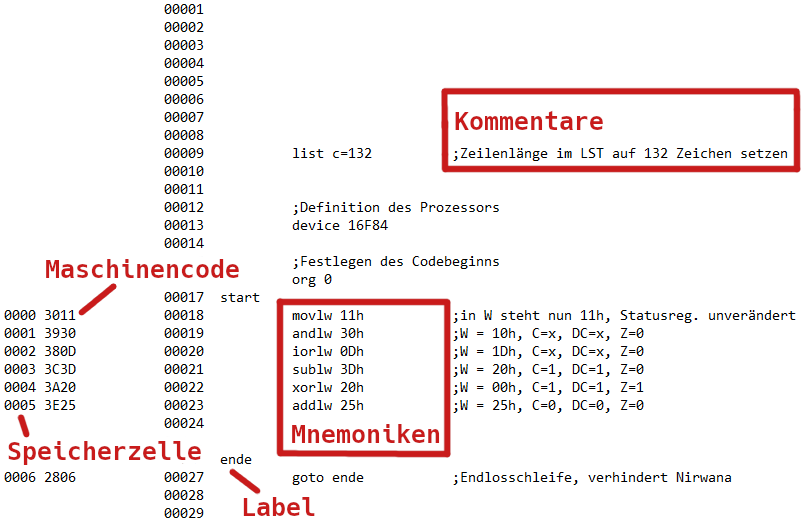
\includegraphics[width=0.8\textwidth]{img/proglisting}
\end{center}

Relevant für die Simulation sind lediglich die ersten zwei Spalten: Speicherzelle und Maschinencode.
Jede Zeile, die keinen Maschinenbefehl enthält, ist aus Sicht der Simulation nicht relevant.
In der Oberfläche des Simulators werden diese Zeilen zwar angezeigt, aber nicht in der Simulation ausgeführt, da sie keine Befehle enthalten.
Beim Durchlaufen des Programms wird der Simulator den jeweiligen nächsten Befehl anzeigen.
Ferner wird der Nutzer die Option haben, Breakpoints zu setzen, d. h. Punkte, an denen die Programmausführung unterbrochen wird.
Schrittweises abarbeiten des Programms wird auch auf Knopfdruck möglich sein.

\subsection{Grafische Benutzeroberfläche}

\begin{center}
    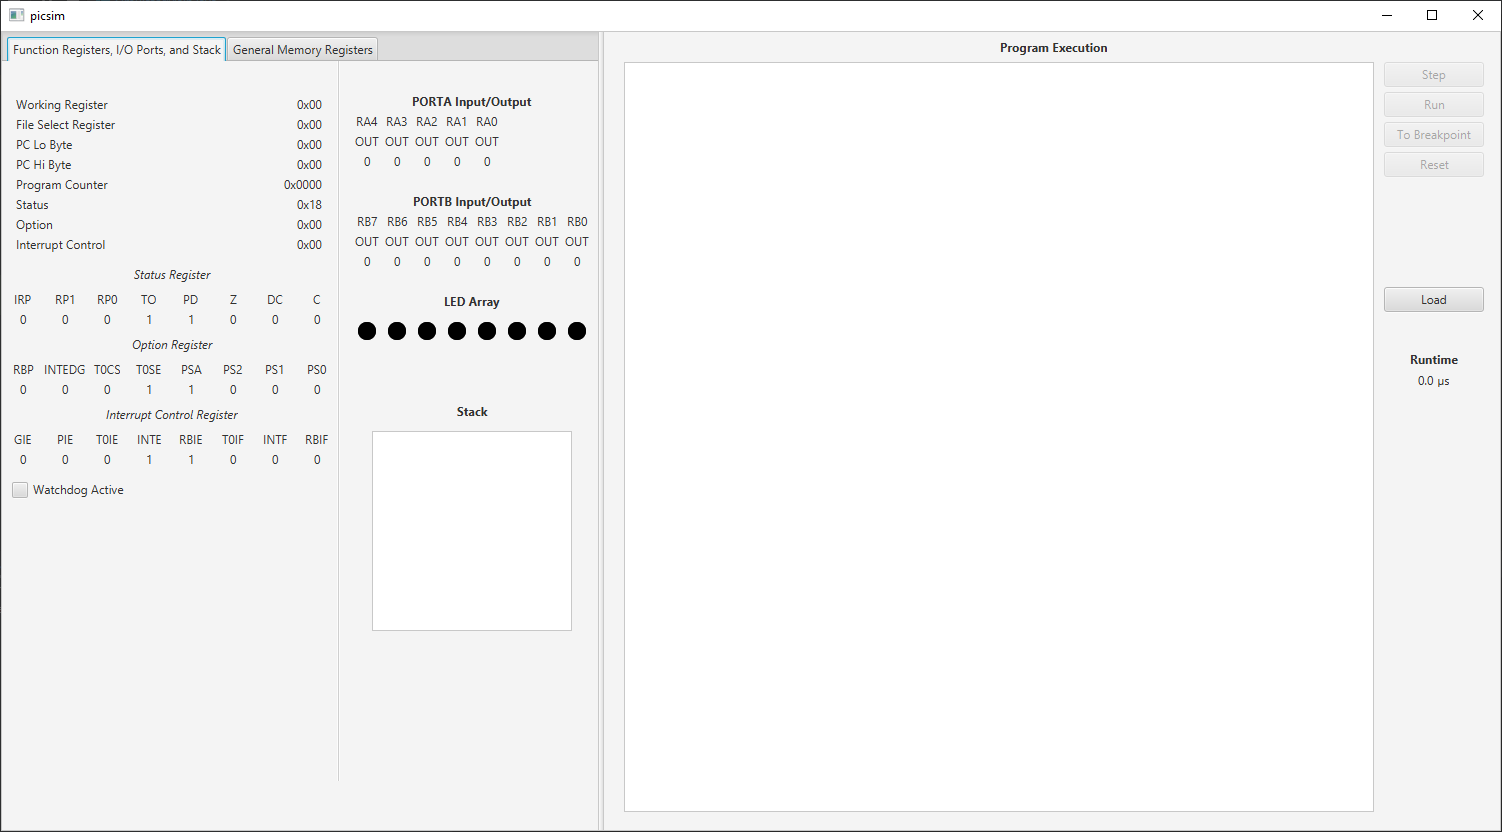
\includegraphics[width=0.8\textwidth]{img/startup}
\end{center}

Die Startoberfläche des Programms ist in zwei Teile aufgeteilt.
Auf der rechten Seite wird ein Codelisting dargestellt, wenn eine Datei geladen wurde.

\begin{center}
    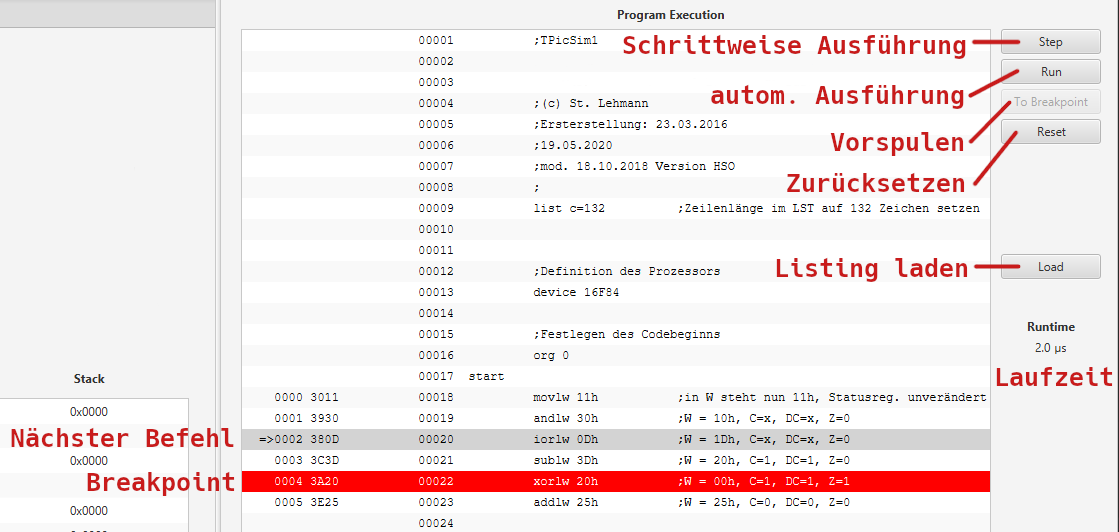
\includegraphics[width=0.7\textwidth]{img/bprunview}
\end{center}

Hier kann der Benutzer den nächsten auszuführenden Befehl sehen, Breakpoints setzen, und den Ausführungsmodus des Programms kontrollieren.
\begin{enumerate}
\item Der Button \texttt{Load} öffnet einen Dateiauswahldialog, in dem ein neues Codelisting ausgewählt und geladen werden kann.
\item Der Button \texttt{Step} läuft in der Simulation einen Schritt weiter.
\item Der Button \texttt{Run} lässt das Programm automatisch weiterlaufen, bis es einen Breakpoint erreicht.
      Dabei werden vier Befehle pro Sekunde durchlaufen. Mit einem weiteren Klick auf den Button kann der Benutzer die automatische Ausführung auch pausieren.
\item Der Button \texttt{To Breakpoint} beschleunigt die automatische Ausführung. In diesem Fall sollte ein Breakpoint gesetzt werden, damit die Ausführung auf dessen Erreichen unterbrochen wird.
\item Im Bereich \texttt{Laufzeit} wird die Prozessorzeit des Mikrocontrollers angegeben (entspricht der Anzahl von Befehlszyklen, die durchlaufen wurden).
\end{enumerate}

Auf der linken Seite gibt es zwei verschiedene Tabs.
Der erste Tab enthält die Darstellung der speziellen Funktionsregister, die Benutzerschnittstelle für die Input/Output-Ports, und die Darstellung des Stacks.

\begin{center}
    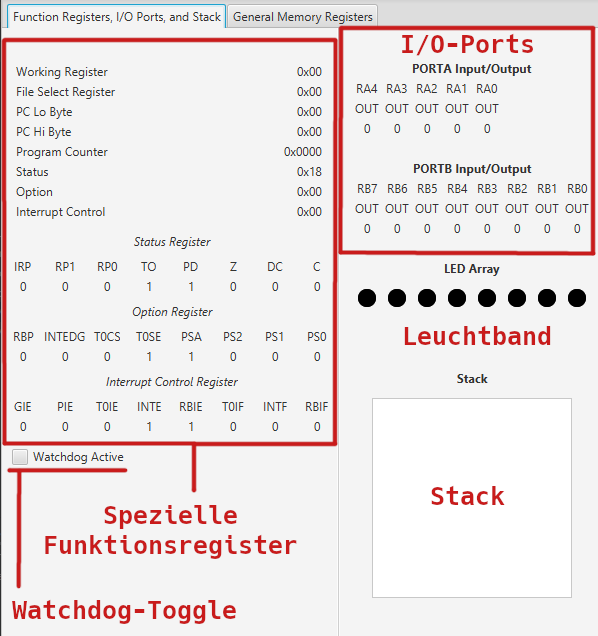
\includegraphics[width=0.6\textwidth]{img/sfrview}
\end{center}

Die linke Seite des Tabs listet die wichtigsten Funktionsregister des Mikrocontrollers und ihre individuellen Werte auf.
Zudem werden Programmzähler und Akkumulator-Register (\textit{Working Register}) dargestellt.
Mit einem Klick auf \texttt{Watchdog Active} kann der Watchdog des Mikrocontrollers aktiviert oder deaktiviert werden.

Auf der rechten Seite werden Input/Output-Ports und der Programmstack dargestellt.
Durck Klicken auf die \texttt{IN}- bzw. \texttt{OUT}-Label kann ein Port auf Ein- bzw. Ausgabemodus gesetzt werden (d. h. der Wert des TRIS-Registers im Mikrocontroller wird verändert).
Steht ein Port auf \texttt{IN}, kann der Wert, der am Port anliegt, durch einen Klick auf die \texttt{1} bzw. \texttt{0} darunter umgestellt werden.
Andernfalls wird der Wert des \texttt{PORTA}- bzw. \texttt{PORTB}-Registers am jeweiligen Bit ausgegeben.

Der zweite Tab gibt eine Übersicht über die allgemeinen Speicherbänke des Mikrocontrollers.
Die Speicherzellen sind ihren Adressen zufolge spaltenweise angeordnet.

\begin{center}
    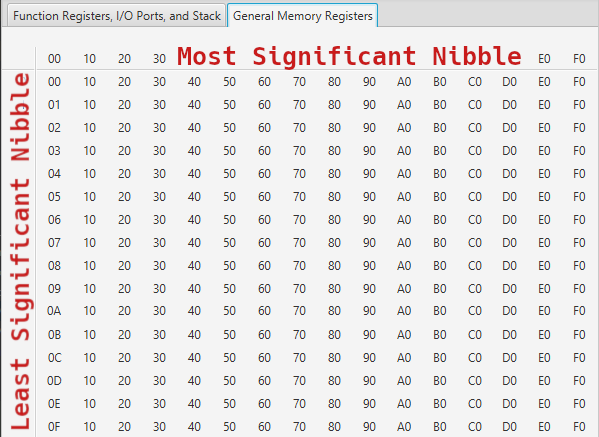
\includegraphics[width=0.5\textwidth]{img/gmrview}
\end{center}

Die Spalten der Tabelle entsprechen folglich dem Wert des \textit{most significant nibble} (die oberen vier Bits der Adresse) und die Zeilen dem \textit{least significant nibble} (die unteren vier Bits).
Um beispielsweise die Adresse \texttt{0x4E} abzulesen, sucht man den Wert in Spalte 5 und Zeile 15.

\section{Entwicklung}

In diesem Abschnitt soll kurz auf die Wahl der Programmiersprache und den Aufbau der Entwicklungsumgebung eingegangen werden.

\subsection{Programmiersprache und UI-Framework}

Als Programmiersprache wurde \textbf{Java} gewählt, eine objektorientierte, imperative Programmiersprache mit einer breiten Menge von Anwendungsbereichen und Bibliotheken.
Java-Software wird auf einer virtuellen Maschine ausgeführt, was die Sprache sehr portierbar macht, da sie auf so gut wie jeder Rechnerplattform läuft.
Das gängigste moderne UI-Framework für Java ist \textbf{JavaFX}, der Nachfolger des Frameworks Swing.
JavaFX bietet diverse Möglichkeiten, um das Aussehen einer Applikation über (F)XML- und CSS-Dateien anzupassen.
So lässt sich mit vergleichsweise wenig Codeaufwand eine ansprechende Benutzeroberfläche konstruieren.

\subsection{Entwicklungsumgebung}

Die App wird über das Buildmanagement-Tool \textbf{Gradle} gebaut.
Gradle erleichtert dem Programmierer die Verwaltung von Abhängigkeiten innerhalb und außerhalb des Projekts und erlaubt es ihm, Prozesse zum Bauen und Testen der Software zu definieren.
Zudem wurde eine Testsuite in \textbf{JUnit} entwickelt, die automatisiert die gegebenen \texttt{LST}-Dateien im Simulator durchlaufen lässt und die Ergebnisse überprüft.
Dies ermöglichte eine sehr effiziente Entwicklung, da Tests für neue Features des Simulators auf Knopfdruck durchgeführt werden konnten.
Der Code wurde über das VCS \textbf{Git} verwaltet und in einem Repository auf der Webseite \textbf{GitHub} gehostet.
Programmiert wurde in der Entwicklungsumgebung \textbf{JetBrains IntelliJ IDEA}, die inzwischen zu einem Standardtool in der Industrie geworden ist.
IDEA bietet einen hohen Grad an Benutzerkomfort und gute Integration mit allen oben genannten Tools.

\section{Implementierung des Simulators}

Im Folgenden soll der Aufbau der App näher erläutert werden.
Neben der grundlegenden Struktur des Backends (dem tatsächlichen Simulator) wird auch die modulare Strukturierung der UI besprochen.

\subsection{Architektur und Entwurfsmuster}

Der \texttt{picsim}-Simulator ist nach dem Entwurfsmuster des \textit{Model-View-Controller} (MVC) aufgebaut.
In diesem Entwurfsmuster arbeitet im Hintergrund der Applikation eine (meist komplexe) Datenstruktur, das \textit{Model}.
Hier ist in diesem Fall die Logik des Simulators implementiert, also u. a. Speicher, Ein- und Ausgabeports und die Logik für Programmausführung und Interrupts.

Das Model wird dem Benutzer der Applikation über den \textit{View} zugänglich gemacht.
Der View ist die strukturierte Darstellung der Daten, die aus dem Model stammen.
Der User kann über Eingaben im View das Model steuern.
Zwischen den beiden sitzt der \textit{Controller}, der Eingaben des Benutzers im View entgegennimmt und entsprechende Veränderungen des Models anstößt.
Diese Veränderungen werden dann wiederum dem Benutzer im View sichtbar gemacht.

\begin{center}
    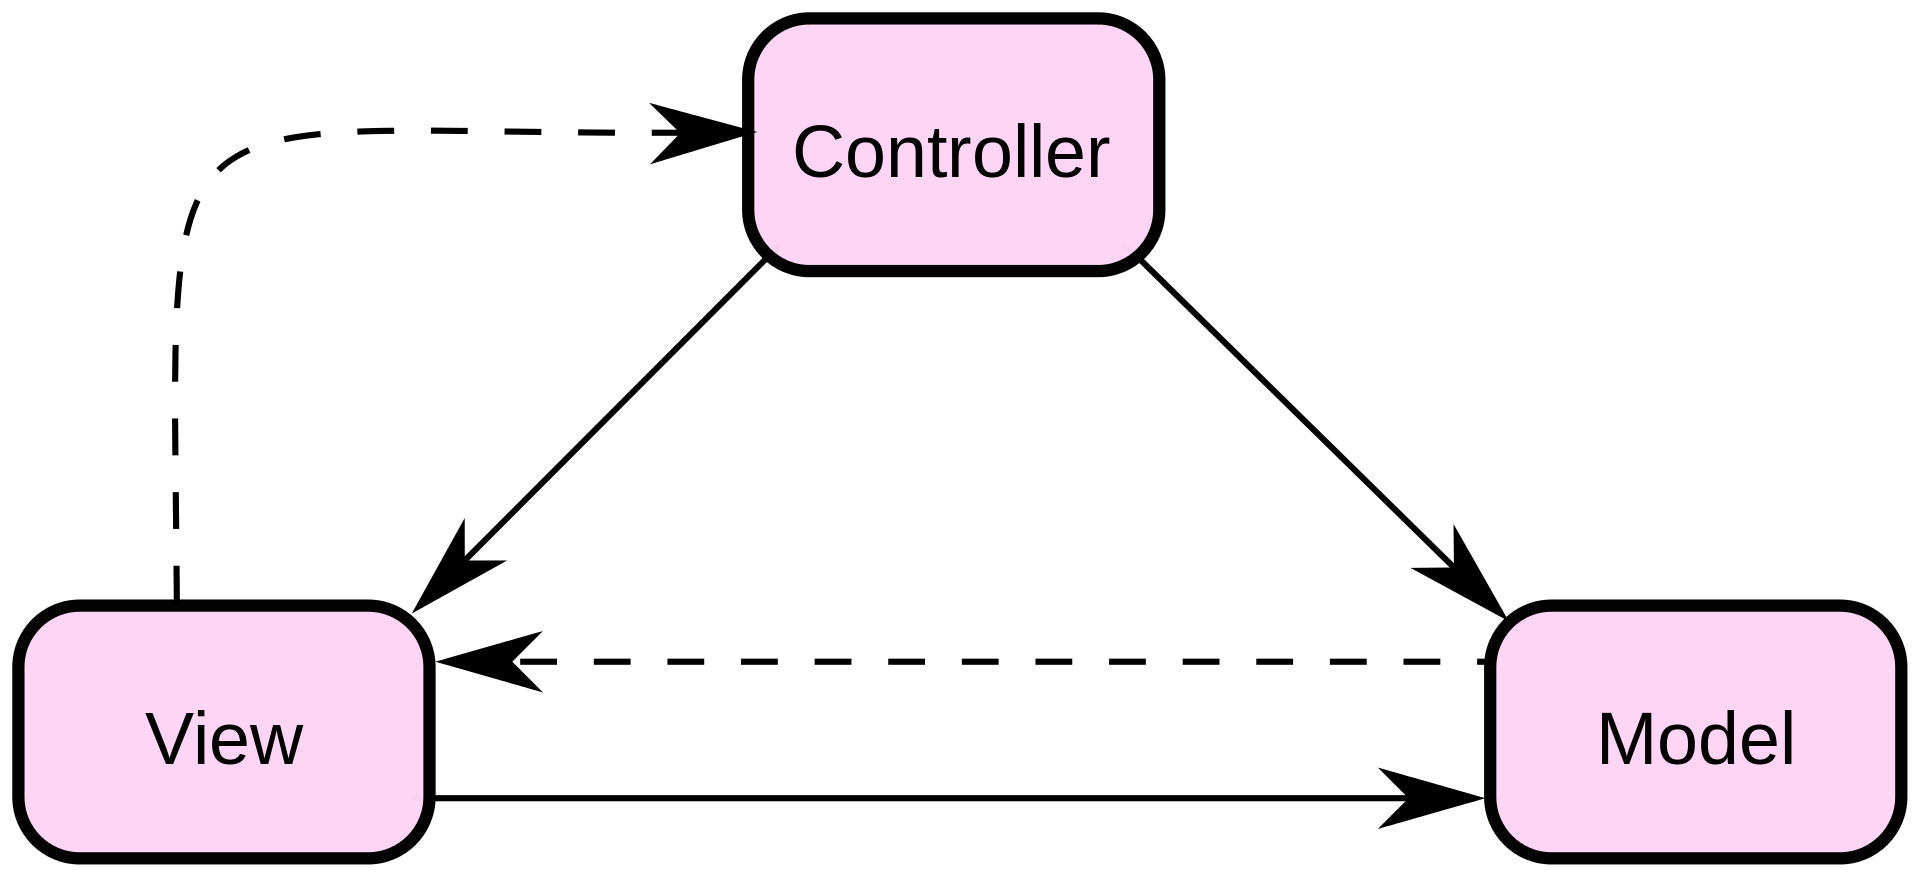
\includegraphics[width=0.4\textwidth]{img/mvcdiag}
\end{center}

\subsection{Klassenstruktur des Models}

Im Model ist die Logik des Mikrocontrollers implementiert.
Über eine Schnittstelle wird eine \texttt{LST}-Datei eingegeben, deren Befehle dann Schritt für Schritt ausgeführt werden.
Dabei bietet das Model Methoden, um interne Daten (Werte in Speicherzellen, Programmzähler, etc.) abzufragen und in den nächsten Zustand überzugehen.
Über diese Schnittstellen kann der Controller bzw. das View dann Zustände abfragen, darstellen, und Übergänge anstoßen.

\begin{center}
    \includegraphics[width=0.8\textwidth]{img/archdiag}
\end{center}

Kernstück des Models ist die Klasse \texttt{Microcontroller}.
Über sie werden alle Daten des Models an das View und den Controller bereitgestellt.
Ein \texttt{Microcontroller} besteht aus folgenden Komponenten:

\begin{itemize}
    \item \texttt{ProgMemory} - Programmspeicher, enthält die Maschinenbefehle, hier realisiert als ein Integer-Array.
    \item \texttt{DataMemory} - Datenspeicher, besteht aus speziellen Funktionsregistern und den allgemeinen Fileregistern, hier realisiert als zwei Integer-Arrays.
    \item \texttt{Stack} - Integer-Array mit einem Stack-Pointer, das bis zu acht 13-Bit Rücksprungadressen eines Programms enthält.
    \item \texttt{IOPins} - Ein- und Ausgabeports des Mikrocontrollers, deren Werte auch in \texttt{DataMemory} abgebildet werden.
    \item \texttt{Watchdog} - Komponente mit separater Taktgebereinheit, die ein Reset-Signal an den Mikrocontroller absetzt, falls eine Zählgrenze überschritten wird.
\end{itemize}

\texttt{DataMemory} enthält zusätzlich noch eine Komponente \texttt{TimerCounter}, die die Logik des internen Timers des Mikrocontrollers nachbildet.
Über sie können auch externe Zähler über den I/O-Port-Eingang \texttt{RB4} angeschlossen werden.

\subsection{Klassenstruktur der Controller und des Views}

JavaFX stellt die View- und Controller-Komponenten des MVC zur Verfügung.
Ein View wird in einer FXML-Datei definiert und besteht aus diversen UI-Widgets, die auf einem Panel angeordnet werden.
In dieser FXML-Datei werden auch Aktionen festgelegt, die im Controller ausgeführt werden, wenn der Benutzer mit diesen UI-Elementen interagiert.
Der Controller ist eine Java-Klasse, die UI-Widgets als Klassenvariablen enthält.
Die Methoden eines Controllers sind Reaktionen auf Benutzereingaben oder -aktivitäten.

Views und Controller sind auch modular aufgebaut.
Das View besteht zwar aus einem Fenster, ist jedoch in einzelne Teile untergliedert.
So sind zum Beispiel das Programmcodefenster, das Fenster für die Funktionsregisterwerte, und die Darstellung des Stacks jeweils in einer separaten FXML-Datei definiert.
Die zugehörigen Controller sind ebenfalls aufgeteilt.
Die Aufteilung der Controller ist in folgendem Klassendiagramm dargestellt.

\begin{center}
    \includegraphics[width=0.8\textwidth]{img/guidiag}
\end{center}

Controller sind für die Aktualisierung ihres jeweiligen Inhalts verantwortlich.
Die Aktualisierung wird jedoch aus dem Hauptcontroller \texttt{SimulatorMain} angestoßen, der die Controller als Klassenvariablen enthält.

\subsection{Implementierung der Interrupts}

Nach jedem Befehlszyklus des Mikrocontrollers wird die Methode \texttt{checkAndHandleInterrupts()} in \texttt{Microcontroller} aufgerufen.
Hier wird überprüft, ob einer der drei möglichen Interrupts ausgelöst wurde und die entsprechenden Bits (GIE und das Enable-Bit des jeweiligen Interrupts) gesetzt sind.
Gesetzt werden die Bits in \texttt{DataMemory} entweder durch die Klasse \texttt{TimerCounter} (beim Überlauf des \texttt{TMR0}-Registers) oder durch \texttt{IOPins} (Flanken auf RB0/INT oder RB4-RB7).

\begin{lstlisting}[language=Java,basicstyle=\ttfamily,columns=fullflexible]
if (this.dataMem.getInterruptRegisterBit(DataMemory.GIE_BIT)) {
    if (t0Interrupt || intInterrupt || rbInterrupt) {

        if (this.poweredDown) {
            this.poweredDown = false;
        }

        this.dataMem.setInterruptRegisterBit(DataMemory.GIE_BIT, false);
        this.stack.push(this.getProgramCounter());
        this.setProgramCounter(DataMemory.ISR_FILE);
    }
} else {
    if (this.poweredDown && (t0Interrupt || intInterrupt || rbInterrupt)) {
        this.poweredDown = false;
    }
}
\end{lstlisting}

Hier sind die \texttt{boolean}-Werte \texttt{t0Interrupt}, \texttt{intInterrupt} und \texttt{rbInterrupt} UND-Verknüpfungen der Enable- und Statusbits der jeweiligen Interrupts.
Stehen beide auf \texttt{1} und ist das GIE-Bit gesetzt, wird der Interrupt ausgelöst.
Beim Auslösen eines Interrupts wird der aktuelle Programmzähler auf den Stack gelegt und die Adresse der \textit{Interrupt Service Routine} (ISR) in den Programmzähler geladen.
Über den \texttt{RETFIE}-Befehl wird an die Adresse zurückgesprungen, an der der Interrupt stattfand.

Ist der Mikrocontroller im \texttt{SLEEP}-Modus, wacht er durch jeden aktiven Interrupt auf (\texttt{this.poweredDown = false}), ohne dass der GIE-Bit gesetzt sein muss.
Die Ausführung wird dann direkt nach dem \texttt{SLEEP}-Befehl fortgesetzt.
Ist der GIE-Bit vor dem \texttt{SLEEP} gesetzt worden, wird wiederum die ISR geladen.
In folgendem Flowchart ist der Ablauf der Abfragen grafisch dokumentiert:

\begin{center}
    \includegraphics[width=0.3\textwidth]{img/intflow}
\end{center}

\subsection{Implementierung des \texttt{TRIS}-Registers}

Die \texttt{TRIS}-Register sind in der Klasse \texttt{IOPins} implementiert.
Die Werte der Register werden in den Variablen \texttt{trisA} und \texttt{trisB} gespeichert.
Soll nun eines der I/O-Register (\texttt{PORTA} oder \texttt{PORTB}) beschrieben werden, muss unterschieden werden, ob der Schreibzugriff intern oder extern ist.
Als Beispiel wird hier die Funktion \texttt{setPortA()} erläutert.

\begin{lstlisting}[language=Java,basicstyle=\ttfamily,columns=fullflexible]
public void setPortA(int portA, boolean external) {
    this.portA = external ? (this.portA & ~this.trisA) + (portA & this.trisA)
                            : (this.portA & this.trisA) + (portA & ~this.trisA);
}
\end{lstlisting}

Wird \texttt{PORTA} vom Mikrocontroller heraus angesprochen (\texttt{external = false}), werden nur die Werte gesetzt, deren Bit in \texttt{TRISA} auf Ausgabe steht.
Soll der Wert hingegen von außerhalb gesetzt werden (über die GUI), so werden nur die Bits berücksichtigt, deren \texttt{TRISA}-Wert auf Eingabe steht.
Mit dem obigen Ausdruck werden die Bitwerte für Ein- bzw. Ausgabe erhalten, während die jeweils anderen aktualisiert werden.

\section{Zusammenfassung}

\subsection{Nachbildung der Funktionalität des PIC16F84}

Mit Ausnahme des EEPROMs wurden die meisten Schlüsselfunktionen des PIC-Bausteins implementiert.
Dabei hat die Implementierung der einzelnen Maschinenbefehle auf Bitebene eine sehr hardwarenahe Abbildung des Speichers ermöglicht.
Die möglichen \textit{Zustände} des PIC bei der Ausführung eines Programms sind also sehr detailgetreu abgebildet.
Abstrakter wird es bei der Implementierung der Logik der einzelnen Bestandteile.
Die Klassenstruktur des Simulator-Backends weist einige Unterschiede zum tatsächlichen Hardwarebaustein auf.
So sind etwa das Bussystem oder ALU anders implementiert, als sie im Blockschaltbild des PIC dargestellt sind.
Die Standardtaktrate des Mikrocontrollers ist 4 MHz, also eine Taktperiode von 0.25 $\mu$s.
Die kleinste Zeitauflösung in der Simulation ist eine Mikrosekunde (ein Befehlszyklus).
Die Timings von Interrupts oder der Timer-Delay wurden somit auch nicht exakt implementiert.
Für die Darstellung der Zustände des Mikrocontrollers zwischen Maschinenbefehlen ist diese Genauigkeit jedoch ausreichend.

\subsection{Fazit}

Die Entwicklung des Projekts ging schnell voran, da wir beide einen fundierten Hintergrund in der Programmierung mit Java haben.
Erste Erfahrungen mit JavaFX waren aufgrund eines Kurses beim dualen Partner auch schon gegeben.
Durch den Software-Engineering-Kurs im dritten und vierten Semester waren auch schon Vorkenntnisse im Umgang mit Versionsverwaltung und Softwaretests vorhanden.

Das anfängliche Konzept mit einer großen Klasse, die eine Vielzahl an Interfaces implementiert, stellte sich nach den ersten Wochen als zu unübersichtlich heraus.
Die Umstellung auf eine modulare Strukturierung des Mikrocontroller-Models war jedoch kein großes Problem, es war lediglich ein Refactoring von einigen Funktionen notwendig.
Ein ähnliches Problem stellte sich beim Aufbau der grafischen Oberfläche heraus: das ursprüngliche FXML, das alle UI-Komponenten des Simulatorfensters enthielt, wurde irgendwann zu groß.
Auch hier bot JavaFX eine komfortable Möglichkeit, die verschiedenen Elemente in unterschiedliche FXML-Dateien aufzusplitten und sie individuell als zusammenhängende Module zusammenzustellen.
Damit ist die Oberfläche des Simulators auch sehr gut erweiterbar und veränderbar.
Genauso konnte auch der Controller von einer großen Klasse in mehrere kleine heruntergebrochen werden.

Die Einrichtung der Unit-Tests in JUnit bedingte zunächst die Definition einer Schnittstelle für die \texttt{Microcontroller}-Klasse.
Sobald diese aber vollständig war, konnte man sehr schnell gute Tests anhand der Test-\texttt{LST}-Dateien entwickeln.
Diese automatisierte Testumgebung hat den Entwicklungsaufwand immens reduziert, da Implementierungsfehler schnell erkannt und beseitigt werden konnten.
Dies war das erste Projekt, wo aufgrund der vorgegebenen Testdaten ein guter Ansatz von \textit{test-driven development} verfolgt werden konnte.
Das Resultat war eine sehr schnelle Entwicklung, die trotz der Geschwindigkeit gute Ergebnisse erzielt hat.

Eventuell könnte man bei einem zukünftigen Projekt die Aufgabenteilung etwas besser machen.
Im aktuellen Projekt waren meist wir beide mit der Lösung eines Problems beschäftigt ("pair programming").
Für die Diskussion von verschiedenen Ansätzen und die Fehlervermeidung durch das Vier-Augen-Prinzip war dieser Ansatz von Vorteil.
Eine Aufteilung der Aufgaben und die separate Bearbeitung wären hier jedoch vermutlich effizienter gewesen.

\end{document}